% Turning points of a one-dimensional potential. Reference: handdraw/ux.png.
% Compile: pdflatex ux_tikz.tex
\documentclass[tikz,border=6pt]{standalone}
\usepackage{amsmath}
\usepackage{fix-cm}
\usetikzlibrary{arrows.meta}
\begin{document}
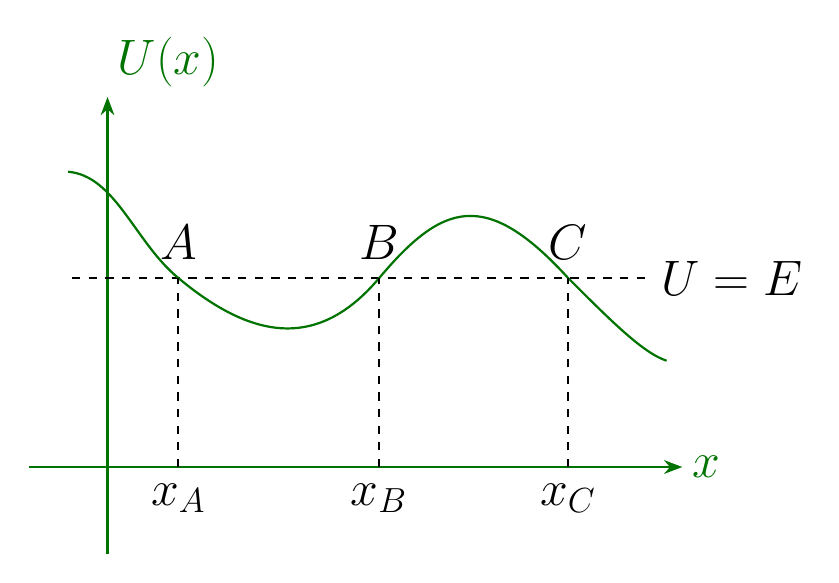
\begin{tikzpicture}[>=Stealth,thick,every node/.style={font=\fontsize{18}{22}\selectfont}]
  \draw[green!45!black,->] (-1,0) -- (7.3,0) node[right] {$x$};
  \draw[green!45!black,->] (0,-1.1) -- (0,4.7) node[above right] {$U(x)$};
  \draw[dashed] (-.45,2.4) -- (6.9,2.4) node[right] {$U=E$};
  \draw[green!45!black] (-.5,3.75)
    .. controls (.1,3.7) and (.35,2.85) .. (.9,2.4)
    .. controls (1.8,1.65) and (2.65,1.45) .. (3.45,2.4)
    .. controls (4.25,3.35) and (4.8,3.55) .. (5.85,2.4)
    .. controls (6.4,1.85) and (6.8,1.45) .. (7.1,1.35);
  \foreach \x/\name in {.9/A,3.45/B,5.85/C} {
    \draw[dashed] (\x,0) -- (\x,2.4);
    \node[above] at (\x,2.5) {$\name$};
    \node[below] at (\x,-.08) {$x_{\name}$};
  }
\end{tikzpicture}
\end{document}
